%%%%%%%%%%%%%%%%%%%%%%%%%%%%%%%%%%%%%%%%%%%%%%%%%%%%%%%%%%%%%%%%%%%%%%%%
%% Customizações do abnTeX2 (http://abnTeX2.googlecode.com)           %%
%% para a Universidade Estadual do Ceara - UECE                       %%
%%                                                                    %%
%% This work may be distributed and/or modified under the             %% 
%% conditions of the LaTeX Project Public License, either version 1.3 %%
%% of this license or (at your option) any later version.             %%
%% The latest version of this license is in                           %%
%%   http://www.latex-project.org/lppl.txt                            %%
%% and version 1.3 or later is part of all distributions of LaTeX     %%
%% version 2005/12/01 or later.                                       %%
%%                                                                    %%
%% This work has the LPPL maintenance status `maintained'.            %%
%%                                                                    %%
%% The Current Maintainer of this work is Thiago Nascimento           %%
%%                                                                    %%
%% Project available on: https://github.com/thiagodnf/uecetex2        %%
%%                                                                    %%
%% Further information about abnTeX2                                  %%
%% are available on http://abntex2.googlecode.com/                    %%
%%                                                                    %%
%%%%%%%%%%%%%%%%%%%%%%%%%%%%%%%%%%%%%%%%%%%%%%%%%%%%%%%%%%%%%%%%%%%%%%%%

%%%%%%%%%%%%%%%%%%%%%%%%%%%%%%%%%%%%%%%%%%%%%%%%%%%%%%%%%%%%%%%%%%%%%%%%
%% Customizações do abnTeX2 (http://abnTeX2.googlecode.com)           %%
%% para a Universidade Estadual do Ceara - UECE                       %%
%%                                                                    %%
%% This work may be distributed and/or modified under the             %% 
%% conditions of the LaTeX Project Public License, either version 1.3 %%
%% of this license or (at your option) any later version.             %%
%% The latest version of this license is in                           %%
%%   http://www.latex-project.org/lppl.txt                            %%
%% and version 1.3 or later is part of all distributions of LaTeX     %%
%% version 2005/12/01 or later.                                       %%
%%                                                                    %%
%% This work has the LPPL maintenance status `maintained'.            %%
%%                                                                    %%
%% The Current Maintainer of this work is Thiago Nascimento           %%
%%                                                                    %%
%% Project available on: https://github.com/thiagodnf/uecetex2        %%
%%                                                                    %%
%% Further information about abnTeX2                                  %%
%% are available on http://abntex2.googlecode.com/                    %%
%%                                                                    %%
%%%%%%%%%%%%%%%%%%%%%%%%%%%%%%%%%%%%%%%%%%%%%%%%%%%%%%%%%%%%%%%%%%%%%%%%

\documentclass[        
    a4paper,          % Tamanho da folha A4
    12pt,             % Tamanho da fonte 12pt
    chapter=TITLE,    % Todos os capitulos devem ter caixa alta
    section=TITLE,    % Todas as secoes devem ter caixa alta
    oneside,          % Usada para impressao em apenas uma face do papel
    english,          % Hifenizacoes em ingles
    spanish,          % Hifenizacoes em espanhol
    brazil            % Ultimo idioma eh o idioma padrao do documento
]{abntex2}

% Importações de pacotes
\usepackage[utf8]{inputenc}                         % Acentuação direta
\usepackage[T1]{fontenc}                            % Codificação da fonte em 8 bits
\usepackage{graphicx}                               % Inserir figuras
\usepackage{amsfonts, amssymb, amsmath}             % Fonte e símbolos matemáticos
\usepackage{booktabs}                               % Comandos para tabelas
\usepackage{verbatim}                               % Texto é interpretado como escrito no documento
\usepackage{multirow, array}                        % Múltiplas linhas e colunas em tabelas
\usepackage{indentfirst}                            % Endenta o primeiro parágrafo de cada seção.
\usepackage{listings}                               % Utilizar codigo fonte no documento
\usepackage{xcolor}
\usepackage{microtype}                              % Para melhorias de justificação?
\usepackage[portuguese,ruled,lined]{algorithm2e}    % Escrever algoritmos
\usepackage{algorithmic}                            % Criar Algoritmos  
%\usepackage{float}                                  % Utilizado para criação de floats
\usepackage{amsgen}
\usepackage{lipsum}                                 % Usar a simulação de texto Lorem Ipsum
%\usepackage{titlesec}                               % Permite alterar os títulos do documento
\usepackage{tocloft}                                % Permite alterar a formatação do Sumário
\usepackage{etoolbox}                               % Usado para alterar a fonte da Section no Sumário
\usepackage[nogroupskip,nonumberlist,acronym]{glossaries}                % Permite fazer o glossario
\usepackage{caption}                                % Altera o comportamento da tag caption
\usepackage[alf, abnt-emphasize=bf, bibjustif, recuo=0cm, abnt-etal-cite=3, abnt-etal-list=0,abnt-etal-text=it]{abntex2cite}  % Citações padrão ABNT
%\usepackage[bottom]{footmisc}                      % Mantém as notas de rodapé sempre na mesma posição
%\usepackage{times}                                 % Usa a fonte Times
\usepackage{mathptmx}                               % Usa a fonte Times New Roman										
%\usepackage{lmodern}                               % Usa a fonte Latin Modern
%\usepackage{subfig}                                % Posicionamento de figuras
%\usepackage{scalefnt}                              % Permite redimensionar tamanho da fonte
%\usepackage{color, colortbl}                       % Comandos de cores
%\usepackage{lscape}                                % Permite páginas em modo "paisagem"
%\usepackage{ae, aecompl}                           % Fontes de alta qualidade
%\usepackage{picinpar}                              % Dispor imagens em parágrafos
%\usepackage{latexsym}                              % Símbolos matemáticos
%\usepackage{upgreek}                               % Fonte letras gregas
\usepackage{appendix}                               % Gerar o apendice no final do documento
\usepackage{paracol}                                % Criar paragrafos sem identacao
\usepackage{lib/uecetex2}		                    % Biblioteca com as normas da UECE para trabalhos academicos
\usepackage{pdfpages}                               % Incluir pdf no documento
\usepackage{amsmath}                                % Usar equacoes matematicas
\usepackage{amsthm}
% Organiza e gera a lista de abreviaturas, simbolos e glossario
\makeglossaries

% Gera o Indice do documento
\makeindex


%%%%%%%%%%%%%%%%%%%%%%%%%%%%%%%%%%%%%%%%%%%%%%%%%%%%%
%%          Configuracoes do ueceTeX2              %%
%%%%%%%%%%%%%%%%%%%%%%%%%%%%%%%%%%%%%%%%%%%%%%%%%%%%%

% Opcoes disponiveis

%\trabalhoacademico{tccgraduacao}
%\trabalhoacademico{tccespecializacao}
\trabalhoacademico{dissertacao}
%\trabalhoacademico{tese}

% Define se o trabalho eh uma qualificacao
% Coloque 'nao' para versao final do trabalho

\ehqualificacao{nao}

% Remove as bordas vermelhas e verdes do PDF gerado
% Coloque 'sim' pare remover

\removerbordasdohyperlink{sim} 

% Adiciona a cor Azul a todos os hyperlinks

\cordohyperlink{nao}

%%%%%%%%%%%%%%%%%%%%%%%%%%%%%%%%%%%%%%%%%%%%%%%%%%%%%
%%          Informação sobre a IES                 %%
%%%%%%%%%%%%%%%%%%%%%%%%%%%%%%%%%%%%%%%%%%%%%%%%%%%%%

\ies{Universidade Estadual do Ceará}
\iessigla{UECE}
\centro{Centro de Ciências e Tecnologia}

%%%%%%%%%%%%%%%%%%%%%%%%%%%%%%%%%%%%%%%%%%%%%%%%%%%%%
%%        Informação para TCC de Graduacao         %%
%%%%%%%%%%%%%%%%%%%%%%%%%%%%%%%%%%%%%%%%%%%%%%%%%%%%%

\graduacaoem{Ciência da Computação}
\habilitacao{bacharel} % Pode colocar tambem 'licenciada'

%%%%%%%%%%%%%%%%%%%%%%%%%%%%%%%%%%%%%%%%%%%%%%%%%%%%%
%%     Informação para TCC de Especializacao       %%
%%%%%%%%%%%%%%%%%%%%%%%%%%%%%%%%%%%%%%%%%%%%%%%%%%%%%

\especializacaoem{Alfabetização de Crianças}

%%%%%%%%%%%%%%%%%%%%%%%%%%%%%%%%%%%%%%%%%%%%%%%%%%%%%
%%         Informação para Dissertacao             %%
%%%%%%%%%%%%%%%%%%%%%%%%%%%%%%%%%%%%%%%%%%%%%%%%%%%%%

\programamestrado{Programa de Pós-Graduação em Ciência da Computação}
\nomedomestrado{Mestrado Profissional em Computação Aplicada}
\mestreem{Ciência da Computação}
\areadeconcentracaomestrado{Ciência da Computação}

%%%%%%%%%%%%%%%%%%%%%%%%%%%%%%%%%%%%%%%%%%%%%%%%%%%%%
%%               Informação para Tese              %%
%%%%%%%%%%%%%%%%%%%%%%%%%%%%%%%%%%%%%%%%%%%%%%%%%%%%%

\programadoutorado{Programa de Pós-Graduação em Saúde Coletiva}
\nomedodoutorado{Doutorado em Saúde Coletiva}
\doutorem{Saúde Coletiva}
\areadeconcentracaodoutorado{Saúde Coletiva}

%%%%%%%%%%%%%%%%%%%%%%%%%%%%%%%%%%%%%%%%%%%%%%
%%  Informação relacionadas ao trabalho     %%
%%%%%%%%%%%%%%%%%%%%%%%%%%%%%%%%%%%%%%%%%%%%%%

\autor{Bruno Bezerra Chaves}
\titulo{MÉTODOS COMBINATORIAIS PARA PROBLEMAS EM REDES DINÂMICAS:
	ALGORITMOS DE AGRUPAMENTO E PREVISÃO DINÂMICOS}
\data{2018}
\local{Fortaleza -- Ceará}

% Exemplo: \dataaprovacao{01 de Janeiro de 2012}
\dataaprovacao{13 de Março de 2017}

%%%%%%%%%%%%%%%%%%%%%%%%%%%%%%%%%%%%%%%%%%%%%
%%     Informação sobre o Orientador       %%
%%%%%%%%%%%%%%%%%%%%%%%%%%%%%%%%%%%%%%%%%%%%%

\orientador{Prof. Dr. Marcos José Negreiros Gomes}
\orientadories{Universidade Estadual do Ceará – UECE}
\orientadorcentro{Centro de Ciências e Tecnologia - CCT}
\orientadorfeminino{nao} % Coloque 'sim' se for do sexo feminino

%%%%%%%%%%%%%%%%%%%%%%%%%%%%%%%%%%%%%%%%%%%%%
%%      Informação sobre o Co-orientador   %%
%%%%%%%%%%%%%%%%%%%%%%%%%%%%%%%%%%%%%%%%%%%%%

% Deixe o nome do coorientador em branco para remover do documento

\coorientador{}
\coorientadories{Universidade Co-orientador - SIGLA}
\coorientadorcentro{Centro do Co-orientador - SIGLA}
\coorientadorfeminino{nao} % Coloque 'sim' se for do sexo feminino

%%%%%%%%%%%%%%%%%%%%%%%%%%%%%%%%%%%%%%%%%%%%%
%%      Informação sobre a banca           %%
%%%%%%%%%%%%%%%%%%%%%%%%%%%%%%%%%%%%%%%%%%%%%

% Atenção! Deixe o nome do membro da banca para remover da folha de aprovacao

% Exemplo de uso:
% \membrodabancadois{Prof. Dr. Fulano de Tal}
% \membrodabancadoisies{Universidade Estadual do Ceará - UECE}

\membrodabancadois{Prof. Dr. Albert Einstein Fernandes Muritiba}
\membrodabancadoiscentro{Centro de Tecnologia - CT}
\membrodabancadoisies{Universidade Federal do Ceará -- UFC}
\membrodabancatres{Membro da Banca Três}
\membrodabancatrescentro{Centro de Ciências e Tecnologia - CCT}
\membrodabancatresies{Universidade do Membro da Banca Três - SIGLA}
\membrodabancaquatro{Membro da Banca Quatro}
\membrodabancaquatrocentro{Centro de Ciências e Tecnologia - CCT}
\membrodabancaquatroies{Universidade do Membro da Banca Quatro - SIGLA}
\membrodabancacinco{Membro da Banca Cinco}
\membrodabancacincocentro{Teste}
\membrodabancacincoies{Universidade do Membro da Banca Cinco - SIGLA}
\membrodabancaseis{Membro da Banca Seis}
\membrodabancaseiscentro{}
\membrodabancaseisies{Universidade do Membro da Banca Seis - SIGLA}

\begin{document}	

	% Elementos pré-textuais
	\imprimircapa
	\imprimirfolhaderosto{}
	%\imprimirfichacatalografica{elementos-pre-textuais/ficha-catalografica}
	%\imprimirerrata{elementos-pre-textuais/errata}
	%\imprimirfolhadeaprovacao
	%\imprimirdedicatoria{elementos-pre-textuais/dedicatoria}
	%\imprimiragradecimentos{elementos-pre-textuais/agradecimentos}
	%\imprimirepigrafe{elementos-pre-textuais/epigrafe}
	\imprimirresumo{elementos-pre-textuais/resumo}
	\imprimirabstract{elementos-pre-textuais/abstract}
	%\imprimirlistadeilustracoes
	%\imprimirlistadetabelas
	%\imprimirlistadequadros
	\imprimirlistadealgoritmos
	%\imprimirlistadecodigosfonte
	%\imprimirlistadeabreviaturasesiglas	
	%\imprimirlistadesimbolos{elementos-pre-textuais/lista-de-simbolos}   
	\imprimirsumario
	
	%Elementos textuais
	\textual
	% \chapter{Introdução}
\chapter{Introdução}
\label{cap:introducao}
Grandes quantidades de dados estão disponíveis para análise em organizações hoje em dia.
Estas enfrentam vários desafios quando se tenta analisar dados gerados com o objetivo de
extrair informações úteis.
Esta capacidade analítica precisa ser reforçada com ferramentas capazes de lidar com
grandes conjuntos de dados sem tornar o processo de análise uma tarefa árdua.
Agrupamento de dados normalmente são usados no processo de análise de dados, pois esta técnica
não exige qualquer conhecimento prévio dos dados. Contudo, os algoritmos de agrupamento
geralmente requerem um ou mais parâmetros de entrada que influenciam o processo de
agrupamento e os resultados que podem ser obtidos. 

Nos últimos anos, o problema de agrupamento dinâmico tem atraído o interesse de pesquisas,
impulsionado pelo aumento da disponibilidade de grandes conjuntos de dados contendo
elementos espaciais e temporais. Este problema pode ser analisado como um problema de
otimização. Seu objetivo principal é maximizar as diferenças das características dos
indivíduos de grupos distintos, e minimizar as diferenças das características dos
indivíduos de um mesmo grupo.


Agrupamento de dados ganhou uso muito difundido, especialmente para dados estáticos.
No entanto, o rápido crescimento de dados espaço-temporais de inúmeros instrumentos,
como os satélites em órbita terrestre, criou uma necessidade de métodos de agrupamento
espaço-temporais para extrair e monitorar clusters dinâmicos. O agrupamento espaço-temporal
dinâmico enfrenta dois grandes desafios: primeiro, os clusters são dinâmicos e podem mudar de
tamanho, forma e propriedades estatísticas ao longo do tempo. Em segundo lugar, vários dados
espaço-temporais são incompletos, ruidosos, heterogêneos e altamente variáveis sobre espaço e tempo.

O problema de agrupamento dinâmico com a componente de previsão divide-se em passos.
A primeira etapa é obtenção das informações espaço-temporais mapeáveis e características do indivíduo.
Neste passo, segue-se três estratégias para resolução do problema: os dados são analisados
como um só grupo (Agrupamento Estático); trata-se os dados por intervalos pré-definidos; e 
mapeamento das evoluções entre intervalos observados. Sendo assim, pretende-se indicar o conjunto
de grupos espacialmente correlacionados também no tempo.

Já o problema de previsão de grupos dinâmicos introduz o conceito de indicar os
possíveis grupos que serão formados no tempo após um conjunto de eventos serem
observados previamente.

O algoritmo proposto para previsão de agrupamentos é uma importante contribuição
deste trabalho, uma vez que poderá ser usado na obtenção de informações, na previsão de movimentação dos grupos e recomendação para o combate a endemias. O serviço proposto se baseia na localização passada dos casos de dengue.


%\section{Caracterização do problema}

\section{Objetivos}
\label{sec:objetivos}
A seguir, são expostos os objetivos desta dissertação, definindo o produto
final a ser obtido.

\subsection{Objetivo Geral}

Estudo e aplicação de métodos existentes e proposta de um método para resolver o Problema de Agrupamento
em Grafos Dinâmicos e previsão de evolução destes agrupamentos.

\subsection{Objetivos Específicos}
\label{sec:objetivos-especificos}

Para que se alcance o objetivo geral, as seguintes metas foram estabelecidas:

\begin{alineas}
	\item Utilizar o software Dynagraph como ambiente de suporte à visualização e interação com os resultados dos métodos de agrupamento espaço-temporal utilizados.
	\item Extração de características de previsão espaço-temporal sobre a evolução dos agrupamentos dinâmicos.
	\item Avaliação dos resultados sobre bases de dados reais ligadas a evolução de casos de Dengue e Chikungunya e outras bases dinâmicas.
\end{alineas}

\section{Hipóteses}
As hipóteses a seguir conduziram a elaboração desta dissertação:
\begin{alineas}
	\item É possível a criação de um algoritmo capaz de sugerir novos agrupamentos geolocalizados baseados no tempo.
	\item É exequível a integração de um editor de características ao DYNAGRAPH, que é um software extensível.
	\item É realizável a utilização do modelo proposto de agrupamentos em grafos dinâmicos em um ambiente Web.
\end{alineas}

\section{Justificativa}
Esta pesquisa justifica-se por perceber-se a necessidade de ferramentas e estudos 
relacionando os assuntos abordados: agrupamento, previsão em dados
dinâmicos espaço-temporais, grafos dinâmicos e sistemas web de forma integrada.
E também, acelerar técnicas de agrupamento em grafos dinâmicos para tomada de decisão.

A relevância da pesquisa está em permitir uma análise dos dados extraídos 
para apoio à tomada de decisão, onde concentra-se na avaliação dos resultados sobre bases de dados
dinâmicas relativas a casos de Dengue.
A pesquisa toma como base as características de evolução dos casos da doença
observados entre 2012 e 2018 em Fortaleza.
Os dados foram tomados a partir de \cite{simda}, onde um estado é definido como o período de uma semana. 

\section{Metodologia}
A seguir, são descritas as etapas metodológicas para o desenvolvimento da dissertação de acordo com o cronograma.

\subsection{Etapas metodológicas do projeto}
A presente pesquisa pode ser caracterizada quanto ao procedimento quantitativa
e comparativa. A pesquisa quantitativa prioriza apontar numericamente a frequência e a
intensidade dos comportamentos dos indivíduos de um determinado grupo, ou população. O
método comparativo constitui-se em investigar coisas ou fatos e explicá-los de acordo com
suas semelhanças e suas diferenças. Possibilita a análise de dados concretos e a dedução de
semelhanças e divergências de elementos contínuos, abstratos e gerais, facilitando investigações
de caráter indireto \cite{fachin}.

\subsubsection{Revisão da literatura e soluções existentes}
As fontes principais de pesquisa foram sites especializados em pesquisas científicas, por exemplo, o portal de periódicos
da CAPES, IEEE e outros sites de referências em que possuem livros, periódicos e dissertações disponíveis.
Os temas essenciais abordados na pesquisa foram:
\begin{itemize}
	\item Estrutura de dados em grafos dinâmicos
	\item Modelos de previsão espaço-temporais
	\item Algoritmos de agrupamentos dinâmicos
\end{itemize}
\subsubsection{Análise de requisitos}
Detectou-se as necessidades de informações baseadas na previsão de agrupamentos dinâmicos
em grafos. Assim sendo, e após obter os dados a partir de \cite{simda}, houve a necessidade de um software para
representação e tratamentos de grafos dinâmicos. Com isso foi escolhido o DYNAGRAPH, que tem como 
característica a extensibilidade.

\subsubsection{Arquitetura do software}
A arquitetura do software desenvolvido é apresentada, assim como o diagrama de caso de uso (UML).

\subsubsection{Modelo e desenvolvimento de software}
Foi desenvolvido um modelo capaz de representar agrupamentos e previsão dinâmicos.
Em seguida, foi desenvolvido a partir do software DYNAGRAPH executar o modelo
proposto e apresentar os resultados para validar a aplicação da ferramenta.

\subsubsection{Ferramentas e Materiais}
O desenvolvimento do trabalho foi realizado a partir dos seguintes equipamentos e materiais:
\begin{itemize}
	\item Macbook Pro 13" modelo 2015 / macOS High Sierra 10.13.2:
	\subitem Processador Intel Core i5 2.7 GHz;
	\subitem Memória de 8GB 1867 MHzs DDR3;
	\subitem HD SSD 128GB;
	\item Ambiente de desenvolvimento Webstorm;
	\item Navegador de internet Google Chrome 63.0.3239.132.
	\item Controle de versão Git (Software e dissertação);
	\item \LaTeX para produção da dissertação;
	\item Portal de periódicos CAPES;
\end{itemize}


\section{Organização do Texto}
Esta dissertação está organizada em 5 capítulos. O capítulo 1 apresenta uma
introdução à necessidade da representação e manipulação do agrupamento espaço-temporal
dinâmico, assim como a previsão da formação de novos grupos dinâmicos.Em seguida são apresentados os objetivos,
hipóteses, a metodologia utilizada e contribuições. O capítulo 2 apresenta a revisão
bibliográfica em modelagem com grafos dinâmicos, métodos de agrupamento por densidade, redes dinâmicas,
o DYNAGRAPH, um editor de características e um conjunto de trabalhos relacionados a esta área do conhecimento.
O capítulo 3 apresenta o modelo de agrupamento e previsão em redes dinâmicas. O capítulo 4 apresenta
os resultados e comparação dos algoritmos apresentados. O capítulo 5 apresenta as considerações finais
e propostas de trabalhos futuros.









	% \chapter{Estado da Arte}
\chapter{Conceitos e revisão bibliográfica}
\label{cap:estadodaarte}

Uma visão geral sobre agrupamentos é apresentada na seção \ref{agrupamentos}. Na seção \ref{dbscan} apresentamos o algoritmo DBSCAN em detalhes e suas características. A seção \ref{stdbscan} apresenta o ST-DBSCAN, que é utilizada nesse trabalho para auxlliar os métodos de previsão dinâmica. Na seção  \ref{redes-dinamicas}  discutimos redes dinâmicas, exibimos o modelo DYNAGRAPH e um editor de características. A seção  \ref{trabalhos-relacionados}  define e apresenta os trabalhos relacionados ao problema de agrupamentos dinâmicos.


\section{Agrupamentos}
\label{agrupamentos}

A técnica de agrupamento, também chamada de clustering, é uma das técnicas de mineração de dados mais comuns e é usada para descobrir padrões de distribuição nos dados. O agrupamento é feito com base na similaridade das características e na posição dos objetos. Dessa maneira, o objetivo é que objetos de mesmo grupo sejam muito similares entre si e muito diferentes dos objetos de outros grupos.

Essa técnica é muito utilizada para dados estáticos. No entanto, há pouco trabalho no âmbito espaço-temporal onde os dados estão na forma de campos espaço-temporais contínuos e os agrupamentos são dinâmicos. Além disso, os dados espaço-temporais originados por satélites em órbita terrestre, telefones celulares e outros sensores tendem a ser ruidosos, incompletos e heterogêneos, tornando sua análise especialmente desafiadora \cite{faghmous2013}.

Agrupamentos dinâmicos podem mudar seu tamanho, forma, localização e propriedades estatísticas de um único passo para o próximo. Embora os agrupamentos possam se mover ou mudar de forma, existem vários pontos que não alteram as associações de grupos por um período de tempo. Tendo isso em vista é possível extrair de forma autônoma agrupamentos dinâmicos em dados espaço-temporais contínuos que podem conter valores, ruídos ou características muito variáveis.

Os métodos mais tradicionais são os particionais e os hierárquicos. Alguns algoritmos de agrupamento integram as idéias de vários outros, logo é difícil classificar um algoritmo pertencendo a somente uma categoria de método de agrupamento. Além do que, algumas aplicações podem ter critérios que necessitam a integração de várias técnicas de agrupamento.  Os principais métodos de agrupamento existentes na literatura podem ser categorizados, como mostra as próximas sessões.

\subsection{Métodos baseados em particionamento}
A ideia principal desta classe de algoritmos de agrupamentos é criar ${K}$ grupos dos dados, onde ${K}$ é inserido pelo usuário.
Esse método consiste em escolher ${K}$ objetos como sendo os centros dos ${K}$ grupos.
Os objetos são divididos entre os ${K}$ grupos de acordo com algum critério de similaridade
estabelecido pelo algoritmo, de modo que cada objeto fique no grupo que tem o menor valor de
distância entre o objeto e o centro dele.
Os algoritmos de particionamento são muito populares devido à sua facilidade de implementação e baixo custo computacional; no entanto, eles têm essas desvantagens: (1) eles são sensíveis à presença de ruído e outliers, (2) eles podem descobrir apenas grupos com formas convexas e (3) o número de grupos precisa ser especificado.

\subsubsection{Agrupamentos K-Médias}
O algoritmo de agrupamento k-médias é uma das técnicas mais populares dessa abordagem e foi introduzido em \cite{Macqueen67}. Ele utiliza a média dos objetos que são do grupo em questão, também conhecido como centro de gravidade do grupo.  A idéia principal neste algoritmo é usar a média dos objetos para atribuí-los a grupos e também usá-los para  representar estes.
K-médias é um algoritmo que garante a convergência para um ótimo local, mas não necessariamente um ótimo global. À medida que ${K}$ aumenta, o custo de encontar a solução ótima diminui, e atinge seu mínimo quando ${K}$ é igual ao número de objetos \cite{Wu2008}. Especificamente, o procedimento é mostrado abaixo:
 \begin{enumerate}
	\item Inserir os objetos para serem agrupados e também o número ${K}$ de grupos.
	\item Escolher aleatoriamente os objetos ${K}$ como centro dos grupos originais.
	\item Atribuir cada objeto ao grupo com a média mais próxima.
	\item Calcular a nova média de cada grupo.
	\item Repetir a partir do passo 3.
	\item Parar quando o critério de convergência estiver satisfeito. Outro critério, mais frequentemente usado, é a minimização do erro quadrático, dado por: 
	\begin{equation}
	E = \sum_{i=1}^{k}\sum_{o\in C_{i}} |o - \mu_{i}|^{2}
	\end{equation}
	onde ${o}$ é o ponto no espaço representando um dado objeto, ${\mu_{i}}$ é o representante do grupo ${C_{i}}$,
	 e ${K}$ o número de grupos.
\end{enumerate}

\subsubsection{Agrupamentos K-Medoids}
O algoritmo de K-Medoids foi introduzido primeiramente em \cite{kaufmann1990} e não é tão sensível aos outliers quanto os k-médias. Nesse algoritmo, cada grupo é representado pelo objeto mais próximo ao centro, conhecido como medoid.
O processo geral para o algoritmo é o seguinte:
 \begin{enumerate}
 	\item Escolher aleatoriamente ${k}$ objetos como os medoids iniciais.
 	\item Atribuir cada um dos objetos restantes ao grupo que possui o medoid mais próximo.
 	\item Em um grupo, selecionar aleatoriamente um objeto que não seja medoid (${nonmedoid}$), que será referenciado como ${O_{nonmedoid}}$.
 	\item Calcular o custo de substituir o medoid com ${O_{nonmedoid}}$. Este custo é a diferença no erro quadrado se o medoid atual for substituído por ${O_{nonmedoid}}$. Se for negativo, faça ${O_{nonmedoid}}$ o medoid do grupo. O erro quadrático é novamente a somado erro de todos os objetos:
 	\begin{equation}
 	E = \sum_{i=1}^{k}\sum_{o\in C_{i}} |o - O_{medoid(i)}|^{2}
 	\end{equation}
 	onde ${O_{medoid(i)}}$ é o medoid do grupo ${i^{th}}$.
 	\item Repetir a partir do passo 2 até que não haja mudanças. 
 \end{enumerate}

\subsection{Métodos hierárquicos}
Nesta classe de algoritmos os objetos são colocados em uma hierarquia que é percorrida de uma forma bottom-up ou top-down para criar os grupos. A vantagem deste tipo de agrupamento é que ele não requer nenhum conhecimento sobre o número de grupos, e sua desvantagem é sua complexidade computacional \cite{Lin2004}. Muitas vezes, uma estrutura em árvore, um dendrograma, é usada para representar os níveis hierárquicos aninhados.

Os aglomerativos funcionam de uma maneira botton-up,
assumindo inicialmente que cada elemento do conjunto de dados representa um grupo. Em seguida, os grupos são fundidos em grupos maiores até a criação de um grupo único ou qualquer outro critério de parada.

A abordagem divisisa trabalham de maneira top-down, considerando todo o conjunto de dados como um só
grupo, que é dividido de maneira recursiva de acordo com a medida de similaridade
estabelecida.

\subsubsection{O algoritmo BIRCH}

Em \cite{Zhang1996}, BIRCH significa Balanced Iterative Reducing and Clustering using Hierarchies e é um algoritmo usado para agrupamentos em bases de dados muito grandes e é considerado um dos métodos hierárquicos mais utilizados na literatura. As vantagens do BIRCH são as seguintes:

\begin{itemize}
	\item BIRCH trabalha de maneira local. Isso é obtido usando medições que indicam a proximidade natural dos pontos, de modo que cada decisão de agrupamento possa ser feita sem verificar todos os pontos de dados ou grupos existentes.
	\item Leva em conta a estrutura de dados espacial. Ele trata os pontos em uma região densa como um único grupo, enquanto os pontos em uma região esparsa são caracterizados como outliers e podem ser removidos opcionalmente.
	\item O algoritmo faz uso total da memória disponível enquanto minimiza os custos de Entrada/saída de dados.
\end{itemize}

Os principais conceitos do BIRCH, que funcionam de maneira incremental, são o Agrupamento por característica(AC) e AC-árvore. Onde AC consiste em todas as informações que precisam ser mantidas sobre um grupo.
Já AC-árvore é utilizada para representar a hierarquia de grupos.
O agrupamento acontece essencialmente em duas fases. Na primeira delas, o algoritmo lê o conjunto de dados e constrói uma AC-árvore inicial.  Essa árvore é utilizada para representar a hierarquia dos grupos. Na segunda fase, um algoritmo de agrupamento selecionado é aplicado às folhas da AC-árvore, removendo grupos esparsos e agrupando os mais densos em grupos maiores.

\subsubsection{O algoritmo CURE}

Em \cite{Guha1998}, um novo algoritmo hierárquico é proposto para detectar grupos que não são necessariamente convexos. Os grupos do CURE são representados por um número fixo de pontos bem espalhados que são encolhidos em direção ao centro do grupo por uma determinada fração. O CURE difere do algoritmo BIRCH de duas maneiras:
\begin{itemize}
\item O CURE começa desenhando uma amostra aleatória em vez de pré-agrupar todos os pontos de dados, como no caso do BIRCH.
\item CURE primeiro particiona a amostra aleatória e, em seguida, em cada partição, os dados são parcialmente agrupados. Em seguida, os outliers são eliminados e os dados pré-agrupados em cada partição são agrupados para gerar os grupos finais.
\end{itemize}
Os resultados experimentais no artigo mostram que o tempo de execução do CURE é sempre menor que o do BIRCH. Mais importante, os resultados mostram que, à medida que o tamanho do banco de dados aumenta, o tempo de execução do BIRCH aumenta rapidamente enquanto o tempo de execução do CURE aumenta muito pouco. O motivo é que o BIRCH varre todo o banco de dados e usa todos os pontos para o pré-agrupamento, enquanto o CURE usa apenas uma amostra aleatória.

\subsection{Métodos baseados em na estrutura de grade}
Enquanto que os outros métodos de agrupamento discutidos são orientados aos dados, os métodos baseados em grade são orientados ao espaço. Essencialmente, o espaço é dividido em células retangulares, representadas por uma estrutura de grade hierárquica.

\cite{Wang1997} propuseram um método de agrupamento baseado em grade, STING (STatistical INformation Grid - Informação estatística baseada em grade), para agrupar bancos de dados espaciais e facilitar consultas orientadas à região. Esse algoritmo se baseia na construção de diversas camadas de grade, onde células de uma camada mais alta são subdivididas para a criação de células nas camadas mais baixas, como mostra a figura \ref{fig:sting}.

\begin{figure}[!h]
	\centering	
	\Caption{\label{fig:sting} Algoritmo STING: subdivisão de células e construção de árvores}	
	\UECEfig{}{
		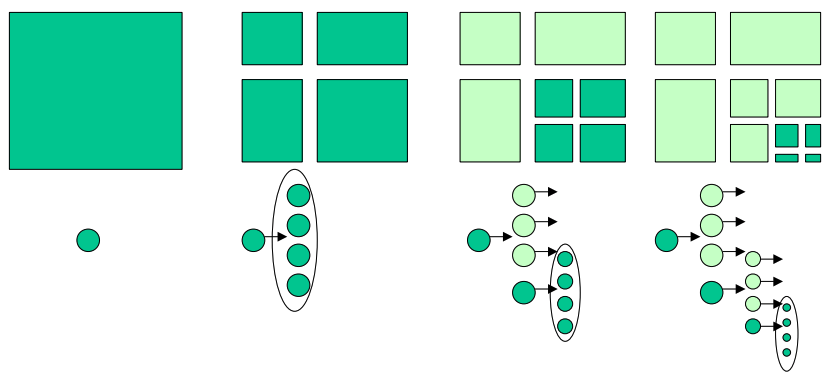
\includegraphics[width=8cm]{figuras/sting.png}
	}{
		\Fonte{\cite{Berkhin2002}}
	}
\end{figure}

O desempenho de STING depende da granularidade do nível mais baixo da estrutura de grade e o resultado dos
grupos são limitados, pois só crescem na horizontal ou vertical e sofrem para buscar grupos de formatos complexos.

Os resultados produzidos pelo STING se aproximam do agrupamento produzido pelo
DBSCAN a medida que a granularidade da estrutura de grade se aproxima de 0, podendo
também ser considerado como um método baseado em densidade.
Uma das vantagens do STING é a complexidade linear de tempo em relação ao número de objetos
a serem agrupados.

\subsection{Métodos baseados em densidade}
Nesta classe de algoritmos, a idéia principal é manter os grupos em crescimento, desde que sua densidade esteja acima de um certo limite. A vantagem dos algoritmos baseados em densidade, em comparação com os algoritmos de particionamento baseados em distância, é que eles podem detectar grupos de forma arbitrária. Isso também fornece uma proteção natural contra outliers. Por outro lado, os algoritmos baseados em distância detectam apenas aglomerados de forma convexa.

Os agrupamentos baseados em densidade analisam a quantidade de elementos dentro de uma vizinhança de acordo com determinados parâmetros. A idéia-chave é que, para cada instância de um grupo, a vizinhança de um determinado raio deve conter pelo menos um número mínimo de instâncias.

A possibilidade de encontrar agrupamentos de forma eventual e o fato de não precisar da definição do número de agrupamentos \cite{yip2005} como parâmetro inicial são as principais vantagens dos métodos baseados em densidade. Entretanto, alguns algoritmos podem exigir a definição de outros parâmetros, como o caso do algoritmo DBSCAN \cite{ESTER1996} abordado na próxima seção.

\section{Método DBSCAN}
\label{dbscan}
% TODO DBSCAN KDD96-037
% TODO O metodo dbscan https://www.maxwell.vrac.puc-rio.br/24787/24787_6.PDF

Este algoritmo calcula a densidade de uma região contando quantos pontos existem em uma determinada área seguindo uma determinada métrica, geralmente uma medida de distância, como a euclidiana ou manhattan. 
É um método efetivo para identificar grupos de formato arbitrário e de diferentes tamanhos, separar os ruídos dos dados, requer apenas um parâmetro de entrada, ajuda o usuário na determinação de um valor apropriado para ele e ajuda a detectar grupos e seus arranjos dentro do espaço de dados, sem qualquer informação preliminar sobre os grupos.
\cite{ESTER1996}  escrevem que a noção de agrupamentos e o algoritmo DBSCAN se aplicam para espaços euclidianos de duas e três dimensões, como para qualquer espaço característico de alta dimensão. O método DBSCAN é aplicável a qualquer base de dados contendo dados de um espaço métrico, isto é, bases de dados com uma função de distância para pares de objetos. Finalmente, o DBSCAN é eficiente mesmo para grandes bancos de dados espaciais.
Para entender o método é necessário conhecer algumas definições específicas listadas a seguir. 

\newtheorem{defDbscan}{Definição}
\begin{defDbscan}
	(Eps-vizinhança de um ponto) Eps-vizinhança de um ponto ${p}$, dado por ${N_{Eps}(p)}$, é definido por ${N_{Eps}(p) = \big\{ q \in D | dist(p, q)  \leqslant Eps\big\} }$. Na figura\ref{fig:epsViz} abaixo os círculos representam respectivamente o Eps-vizinhança do ponto ${q}$ e Eps-vizinhança do ponto ${p}$. Uma abordagem ingênua poderia exigir para cada ponto em um cluster que haja pelo menos um número mínimo (MinPts) de pontos na Eps-vizinhança daquele ponto. No entanto, esta abordagem falha porque há dois tipos de pontos em um grupo, pontos dentro do grupo (centrais) e pontos na fronteira do grupo (pontos de borda). 
\end{defDbscan}

\begin{figure}[!h]
	\centering
	\Caption{\label{fig:epsViz} Eps-vizinhança de  ${q}$ e Eps-vizinhança de ${p}$}	
	\UECEfig{}{
		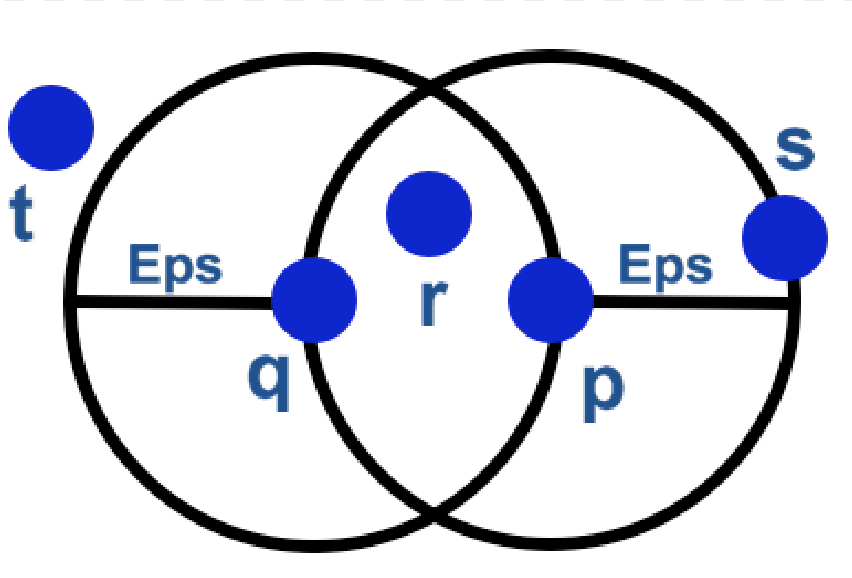
\includegraphics[width=8cm]{figuras/epsViz.png}
	}{
		\Fonte{Elaborado pelo autor}
	}
\end{figure}

\begin{defDbscan}
	(Ponto Central) : Se o Eps-vizinhança de um objeto ${p}$ contém ao menos um número mínimo, MinPts, de objetos, então o objeto ${p}$ é chamado de ponto central.
	Por exemplo, na figura \ref{fig:epsViz}, se adotarmos MinPts = 4, p é um ponto central e os demais não são pontos centrais.
\end{defDbscan}







 O método DBSCAN separa os pontos de dados em três classes:
• Pontos principais. Estes são pontos que estão no interior de um cluster. Um ponto é um ponto interior se houver pontos suficientes em sua vizinhança.
• Pontos de fronteira. Um ponto de fronteira é um ponto que não é um ponto central, ou seja, não há pontos suficientes em sua vizinhança, mas ele está dentro da vizinhança de um ponto central.
• Pontos de ruído. Um ponto de ruído é qualquer ponto que não é um ponto central ou um ponto de fronteira.

Para encontrar um cluster, o DBSCAN começa com uma instância arbitrária (p) no conjunto de dados (D) e recupera todas as instâncias de D em relação a Eps e MinPts
Density-Based Algorithms for Discovering Clusters in Large Spatial Databases with Noise (DBSCAN)
DBSCAN [1] é um algoritmo baseado em densidade que descobre clusters com forma arbitrária e com um número mínimo de parâmetros de entrada. Os parâmetros de entrada necessários para este algoritmo são o raio do cluster (Eps) e os pontos mínimos necessários dentro do cluster (Minpts).

2.2. Descrição do Algoritmo
Nesta seção, o algoritmo DBSCAN [7] Clustering espacial baseado em densidade de aplicativos com ruído é projetado para descobrir os clusters de dados espaciais com ruído. As etapas envolvidas neste algoritmo são as seguintes,
…
(i) Selecione um ponto arbitrário p
(ii) Recuperar todos os pontos de densidade-reachable de p w.r.t. Eps e Minpts.
(iii) Se p é um ponto central, um cluster é formado.
(iv) Se p é um ponto de borda, nenhum ponto é densidade acessível de p e DBSCAN visita o próximo ponto do banco de dados.
(v) Continue o processo até que todos os pontos tenham sido processados.

2.3 Impacto do Algoritmo
DBSCAN requer dois parâmetros de entrada (pontos mínimos e raio) e suporta o usuário ao encontrar um valor aproximado para ele usando o gráfico k-dist [7]. Ele descobre grupos de forma arbitrária. Ele é válido para grandes bancos de dados espaciais.
…

2.4 Trabalho futuro
O algoritmo DBSCAN aqui considera [1] apenas objetos de ponto, mas pode ser estendido para outros objetos espaciais, como polígonos. As aplicações do DBSCAN para espaços de recursos de alta dimensão devem ser investigadas e a geração de raio para esses dados de alta dimensão também precisa ser explorada. Também não consegue detectar agrupamentos com densidade variada.

% Dissertação_AntonioCavalcanteAraujoNeto_Final
DBSCAN (Density-based Spatial Clustering of Applications with Noise) é um algoritmo
de agrupamento baseado em densidade vastamente utilizado pela comunidade científica.
Seu objetivo principal consiste em encontrar concentrações de elementos que estão espacialmente
próximos. Em outras palavras, o algoritmo busca por pontos que possuem mais que um
limiar de vizinhos dentro de um certo raio. Caso um elemento p satisfaça essa propriedade, os
vizinhos de p pertencerão ao mesmo cluster que p e o mesmo processo é aplicado a todos os
seus vizinhos. Além do conjunto de dados a ser agrupado, o DBSCAN recebe também dois
parâmetros de entrada: minPoints e eps. O primeiro deles se refere à quantidade mínima de
pontos em um certo raio de vizinhança para a formação de um cluster. Já o segundo parâmetro
se refere ao raio no qual a verificação de vizinhança é realizada. A função de distância utilizada
para determinar a vizinhança de um certo ponto é definida de acordo com o tipo de dado
a ser agrupado e deve obedecer às restrições de uma função de distância, tais como simetria
e a desigualdade triangular, além de assumir que a distância entre dois elementos x e y só é
igual a 0 se x = y. Dentre suas vantagens, o algoritmo DBSCAN se destaca por ser capaz de
encontrar clusters com formatos arbitrários, além de ser capaz de lidar com ruídos nos dados,
característica que não está presente na maioria dos algoritmos de agrupamento, como mostrado
na Figura 2.1.
As definições básicas utilizadas no DBSCAN são apresentadas a seguir:
• |A|: cardinalidade do conjunto A.
• Neps(p): é o conjunto de pontos q que estão a uma distância menor que eps do ponto p.
Também é chamado de conjunto dos vizinhos de p.
• Diretamente alcançável por densidade (DDR): um ponto p é DDR a partir de um ponto q
se p E Neps(q) e |Neps(q)| >= minPoints.

Figura 2.1: Clusters de formatos arbitrários encontrados pelo algoritmo DBSCAN
Fonte: Data Mining - The Hypertextbook
• Alcançável por densidade (DR): um ponto p é DR a partir de um ponto q, se existe uma
sequência de pontos {p1,..., pn} onde p1 = p e pn = q, tal que pi+1 é DDR a partir de pi
.
• Conectado por densidade (DC): Um ponto p está conectado por densidade a um ponto q
se existe um ponto o tal que p e q são DR a partir de o.
• Core point: um ponto p é classificado como core point se |Neps(o)| >= minPoints.
• Border point: um ponto p é classificado como border point se |Neps(p)| < minPoints e p
é DDR a partir de um core point.
• Noise: Um ponto p é classificado como noise se |Neps(q)| < minPoints e p não é DDR a
partir de nenhum core point.
No contexto do algoritmo DBSCAN, um cluster C é definido como um subconjunto
não vazio dos dados que satisfaz as seguintes propriedades:
• Maximalidade: Para quaisquer dois pontos p e q, se p E C e q é alcançável por densidade
(DR) a partir de p, então q E C.
• Conectividade: Para quaisquer dois pontos p,q E C, p é q são conectados por densidade
(DC).
O Algoritmo 1 mostra o pseudocódigo do DBSCAN. Para cada elemento p ainda
não visitado o conjunto dos seus vizinhos Neps(p) é encontrado, como podemos ver entre as linhas
2 e 5. Caso a cardinalidade desse conjunto de vizinhos seja maior que o valor de minPoints
(Linha 6 do Algoritmo), um novo cluster C é criado e p e seus vizinhos serão atribuídos a C.
Ainda, os pontos não visitados de C serão expandidos em um processo similar. A agrupamento
acaba quando todos os elementos do conjunto foram visitados.
O Algoritmo 2 implementa a função de expansão de um cluster C. A expansão
de um cluster a partir de um ponto p encontra todos os elementos que são conectados por
densidade (DC) a p. Essa função recebe como entrada p, seu conjunto de vizinhos NeighborPts,
o identificador C do cluster a ser expandido, e os parâmetros eps e minPoints. Para cada ponto
p' do conjunto de vizinhos de p, caso esse ponto ainda não tenha sido visitado, sua vizinhança
é recuperada e adicionada ao conjunto NeighborPts de vizinhos que serão verificados (linha
8). Após sua verificação, caso p' não pertença a nenhum cluster, ele é adicionado ao cluster C
(linhas 11 a 13). O processo finaliza quando o conjunto NeighborPts está vazio.

Alg 1 e alg 2

Como podemos ver nos Algoritmos 1 e 2, a complexidade do DBSCAN depende
diretamente do custo computacional para recuperação da vizinhança de um ponto (linhas 7 e
6 dos Algoritmos 1 e 2, respectivamente). Em uma solução ingênua essa operação poderia ser
executada em tempo linear, onde uma simples busca exaustiva em todo o conjunto de dados
retornaria apenas os elementos a uma certa distância do ponto de consulta. Tal solução faria
com que a complexidade do algoritmo DBSCAN fosse O(n2). Por outro lado, com o auxílio
de estruturas de índices, como k-d-Trees ou R-Trees, a complexidade do DBSCAN pode ser
significantemente reduzida. Recentemente foi provado em (GAN; TAO, 2015) que para dimensões
maiores que 2 o algoritmo DBSCAN executa em uma complexidade Omega(n4/3). No entanto,
consideraremos nesse trabalho conjuntos de dados de apenas duas dimensões.



Para agrupar os pontos levando em conta o fator tempo é necessário uma alteração no algoritmo DBScan, e com isso detectar os grupos em relação ao tempo. Logo, o algoritmo determinada para esta implementação foi o ST-DBScan \cite{Birant2007STDBSCANAA}, abordado a seguir.

\section{Método ST-DBSCAN}
\label{stdbscan}
% Spatial- Temporal Density Based Clustering (ST-DBSCAN)

6.1. Introdução

O algoritmo ST-DBSCAN é construído modificando o algoritmo DBSCAN [7]. Em contraste com o algoritmo de agrupamento baseado em densidade existente, o algoritmo ST-DBSCAN [12] tem a capacidade de descobrir clusters em relação aos valores não espaciais, espaciais e temporais dos objetos. As três modificações feitas no algoritmo DBSCAN são as seguintes,

(i) O algoritmo ST-DBSCAN pode agrupar dados espaciais-temporais de acordo com atributos não espaciais, espaciais e temporais.
(ii) DBSCAN não detecta pontos de ruído quando é de densidade variada, mas isso o algoritmo supera esse problema ao atribuir o fator de densidade a cada cluster.
(iii) Para resolver os conflitos em objetos de borda, ele compara o valor médio de um cluster com o novo valor que vem.

6.2. Descrição do Algoritmo
O algoritmo começa com o primeiro ponto p no banco de dados D.
(i) Este ponto p é processado de acordo com o algoritmo DBSCAN e o próximo ponto é tomado.
(ii) A função RetrieveNeighbors (objeto, Ep1, Ep2) recupera todos os objetos densidade-acessível do objeto selecionado em relação a Eps1, Eps2 e Minpts. Se os pontos devolvidos no Eps-neighborhood são menores do que Minpts, o objeto é atribuído como ruído.
(iii) Os pontos marcados como ruído podem ser alterados posteriormente, e os pontos não são diretamente acessíveis, mas serão densidade-acessível.
…
(iv) Se o ponto selecionado for um objeto central, um novo cluster será construído. Então, todos os vizinhos de densidade direta de este núcleo de objetos também estão incluídos.
(v) Então, o algoritmo coleta de forma iterativa objetos atingidos pela densidade do objeto do núcleo usando a pilha.
(vi) Se o objeto não estiver marcado como ruído ou não estiver em um cluster e a diferença
entre o valor médio do cluster e o novo valor é menor do que DeltaE, ele é colocado no cluster atual.

\section{Redes dinâmicas}
 \label{redes-dinamicas} 
\subsection{O modelo Dynagraph}
\subsection{Editor de características}
\section{Trabalhos Relacionados}
 \label{trabalhos-relacionados} 
Como há uma carência de estudos relacionando os assuntos abordados: agrupamento,
previsão em dados dinâmicos espaço-temporais, grafos dinâmicos e sistemas web
de forma integrada, foi necessário dividir o problema de agrupamentos e previsões dinâmicos em três etapas:
\begin{itemize}
\item Estrutura de dados em grafos dinâmicos
\item Modelos de previsão espaço-temporais
\item Algoritmos de agrupamentos dinâmicos
\end{itemize}

A pesquisa aborda estrutura de dados em grafos dinâmicos usando passos já descritos na literatura,
principalmente o modelo Dynagraph \cite{dynagraph}, que é baseado na primeira proposta
em \cite{dynagraph2012}, onde o Dynagraph usa sequências temporais para vértices, arestas,
características modificáveis dos vértices e arestas e o relacionamento entre suas características.
Com isso, é formado um grafo com as informações necessárias para qualquer instante no tempo.
O Dynagraph é capaz de visualizar o comportamento do grafo ao longo de um período de tempo,
e editá-lo.

A ideia central de \cite{kim} é modelar uma rede dinâmica como digrafos orientados ao
tempo (\textit{time-ordered graph}), que é gerada através da ligação de instantes temporais com arestas
direcionadas que unem cada nó ao seu sucessor no tempo. Com isso, transformar uma rede dinâmica
em um grafo maior, mas facilmente analisável. Isto permite não só a utilização dos algoritmos 
desenvolvidos para grafos estáticos, mas também para melhor definir métricas para grafos dinâmicos.
Segundo \cite{kim} um sistema de grafos dinâmicos é um objeto de representação visual
que pode descrever melhor o comportamento dinâmico de objetos relacionados a eventos dinâmicos e
introduzir novas formas de enxergar ou descrever a evolução de eventos dinâmicos na natureza.

\cite{kostakos} considera a estrutura de grafos temporais como grafos
estáticos, no entanto avança sobre as métricas introduzindo conceitos como disponibilidade
temporal, proximidade temporal e geodésica, e estuda os seus grafos sobre redes reais.

Segundo \cite{density-based-clusters}, o algoritmo DBScan(\textit{Density-Based Spatial Clustering
of Applications With Noise}) calcula a densidade de uma região contando quantos pontos existem
em uma determinada área seguindo uma determinada métrica. Ele permite a redução de pontos não
pertencentes a nenhum padrão, assim como possibilita a formação de grupos de diferentes formas.
Seu objetivo principal é dividir os pontos em grupos através da densidade de cada região.

\cite{lahiri2007} apresentam um algoritmo de predição em redes temporais, e que usa a ideia de que certas
interações sinalizam a ocorrência de outros em algum momento no futuro. Através de análises estatísticas
o algoritmo mede o atraso entre as interações, e com isso pode-se prever quando certas interações vão ocorrer
com base em observações passadas e atuais. Propõe-se a utilização de subgrafos frequentes e discute
como identificar subgrafos que são persistidos em redes temporais.
\cite{lahiri2008} em seguida propõe um novo problema de mineração de dados para redes dinâmicas:
detecção de todos os padrões de interação que ocorrem em intervalos de tempo regulares.

% \cite{alfredo} propôs um algoritmo baseado no método IGN (Identificador
% de Grupos Naturais) de \cite{simposioNeg}, onde este apresenta bons resultados tanto para distâncias 
% euclidianas quanto para outras distâncias; é sensível à presença de \textit{outliers} em situações muito específicas;
% e o número de grupos naturais e sua composição é obtida automaticamente no processo.
% A pesquisa seguirá este método para verificar o processo de construção de agrupamentos dinâmicos.











	\chapter{Fundamentação Teórica}
\label{cap:fundamentacao-teorica}

	\chapter{Trabalhos Relacionados}
\label{cap:trabalhos-relacionados}

Integer non lacinia magna. Aenean tempor lorem tellus, non sodales nisl commodo ut. Proin mattis placerat risus sit amet laoreet. Praesent sapien arcu, maximus ac fringilla efficitur, vulputate faucibus sem. Donec aliquet velit eros, sit amet elementum dolor pharetra eget. Integer eget mattis libero

\section{Trabalho Relacionado A}
\label{sec:trabalho-relacionado-a}

\lipsum[10]

	\begin{figure}[h!]
		\centering
		\Caption{\label{fig:exemplo-1} Lorem ipsum dolor sit amet, consectetur adipiscing elit. Suspendisse commodo lectus et augue elementum varius.}	
		\UECEfig{}{
			\fbox{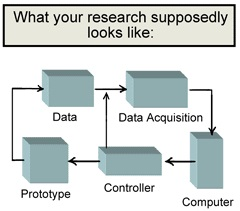
\includegraphics[width=8cm]{figuras/figura-1}}
		}{
			\Fonte{Elaborado pelo autor}
		}	
	\end{figure}
	
\lipsum[11]

\section{Trabalho Relacionado B}
\label{sec:trabalho-relacionado-b}

Integer non lacinia magna. Aenean tempor lorem tellus, non sodales nisl commodo ut. Proin mattis placerat risus sit amet laoreet. Praesent sapien arcu, maximus ac fringilla efficitur, vulputate faucibus sem. Donec aliquet velit eros, sit amet elementum dolor pharetra eget. Integer eget mattis libero. Praesent ex velit, pulvinar at massa vel, fermentum dictum mauris. Ut feugiat accumsan augue, et ultrices ipsum euismod vitae

	\begin{figure}[h!]
		\centering
		\Caption{\label{fig:exemplo-2} Maecenas luctus augue odio, sed tincidunt nunc posuere nec}	
		\UECEfig{}{
			\fbox{
\includegraphics[width=8cm]{figuras/figura-2}}
		}{
			\Fonte{Elaborado pelo autor}			
		}	
	\end{figure}

Nunc ac pretium dui. Mauris aliquam dapibus nulla ac mattis. Aenean non tortor volutpat, varius lectus vitae, accumsan nibh. Cras pretium vestibulum enim, id ullamcorper tortor ultrices non. Integer sodales viverra faucibus. Curabitur at dui lacinia, rhoncus lacus at, blandit metus. Integer scelerisque non enim quis ornare.

	\begin{quadro}[h!]	
		\centering
		\Caption{\label{qua:exemplo-1} Praesent ex velit, pulvinar at massa vel, fermentum dictum mauris. Ut feugiat accumsan augue}		
		\UECEqua{}{
			\begin{tabular}{|c|c|l|l|}
				\hline
				Quisque & pharetra & tempus & vulputate \\
				\hline
				E1 & Complete coverage by a single transcript & Both  & Complete\\
				\hline
				E2 & Complete coverage by more than & Both splice sites & Complete\\
				\hline
				E3 & Partial coverage & Both splice sites & Both \\				
				\hline
			\end{tabular}
		}{
			\Fonte{Elaborado pelo autor}
		}
	\end{quadro}
	
\lipsum[20]

	
	\begin{quadro}[h!]	
		\centering
		\Caption{\label{qua:exemplo-2} Duis faucibus, enim quis tincidunt pellentesque}		
		\UECEqua{}{
			\begin{tabular}{|c|c|}
				\hline
				Quisque & pharetra \\
				\hline
				E1 & Complete coverage by a single transcript \\
				\hline
				E2 & Complete coverage by more than \\
				\hline
				E3 & Partial coverage \\
				\hline
				E4 & Partial coverage \\
				\hline
				E5 & Partial coverage \\
				\hline
				E6 & Partial coverage \\
				\hline
				E7 & Partial coverage \\
				\hline
			\end{tabular}
		}{
			\Fonte{Elaborado pelo autor}
		}
	\end{quadro}

\lipsum[21]

Integer non lacinia magna. Aenean tempor lorem tellus, non sodales nisl commodo ut. Proin mattis placerat risus sit amet laoreet. Praesent sapien arcu, maximus ac fringilla efficitur, vulputate faucibus sem. Donec aliquet velit eros, sit amet elementum dolor pharetra eget. Integer eget mattis libero.
\Gls{ambiguidade}
\Gls{braile}
\Gls{coerencia}
\Gls{dialetos}
\Gls{elipse}
\Gls{locucao-adjetiva}
\Gls{modificadores}
\Gls{paronimos}
\Gls{sintese}
\Gls{borboleta}
	\chapter{Metodologia}
\label{chap:metodologia}

\lipsum[2]
\lipsum[12]

O autor \cite{lamport1986latex} e \cite{Maia2011} \lipsum[2] 

\begin{table}[h!]
	\Caption{\label{tabela-ibge} Um Exemplo de tabela alinhada que pode ser longa ou curta, conforme padrão IBGE. conforme padrão IBGE. conforme padrão IBGE. conforme padrão IBGE. conforme padrão IBGE. conforme padrão IBGE. conforme padrão IBGE. conforme padrão IBGE. conforme padrão IBGE. conforme padrão IBGE. conforme padrão IBGE.}%
	\IBGEtab{}{%
		\begin{tabular}{ccc}
			\toprule
			Nome & Nascimento & Documento \\
			\midrule \midrule
			Maria da Silva & 11/11/1111 & 111.111.111-11 \\
			Maria da Silva & 11/11/1111 & 111.111.111-11 \\
			Maria da Silva & 11/11/1111 & 111.111.111-11 \\
			\bottomrule
		\end{tabular}%
	}{%
	\Fonte{Produzido pelos autores}%
	\Nota{Esta éuma nota, que diz que os dados são baseados na
		regressão linear.}%
	\Nota[Anotações]{Uma anotação adicional, seguida de várias outras.}%
}
\end{table}

\cite{Huetal2000} \lipsum[2] 

\section{Exemplo de Algoritmos e Figuras}
\label{sec:exemplo-de-algoritmos-e-figuras}

\lipsum[2]

\begin{algorithm}[h!]
	\SetSpacedAlgorithm
	\caption{\label{exemplo-de-algoritmo}Como escrever algoritmos no \LaTeX2e}
	\Entrada{o proprio texto}
	\Saida{como escrever algoritmos com \LaTeX2e }
	\Inicio{
		inicializa\c{c}\~ao\;
		\Repita{fim do texto}{
			leia o atual\;
			\Se{entendeu}{
				vá para o próximo\;
				próximo se torna o atual\;}
			\Senao{volte ao início da seção\;}
		}
	}	
\end{algorithm}

\lipsum[2]
%\begin{algorithm}[H]
%	\Entrada{o proprio texto}
%	\Saida{como escrever algoritmos com \LaTeX2e }
%	\Inicio{
%		inicializa\c{c}\~ao\;
%		\Repita{fim do texto}{
%			leia o atual\;
%			\Se{entendeu}{
%				vá para o próximo\;
%				próximo se torna o atual\;}
%			\Senao{volte ao início da seção\;}
%		}
%	}
%	\caption{Exemplo de Algoritmo Versao 02}
%\end{algorithm}

%\begin{algorithm}
%	\begin{algorithmic}
%	\Entrada{o proprio texto}
%	\Saida{como escrever algoritmos com \LaTeX2e }	
%	\end{algorithmic}
%\end{algorithm}

Exemplo de alíneas com números:

\begin{alineascomnumero}
	\item Lorem ipsum dolor sit amet, consectetur adipiscing elit. Nunc dictum sed tortor nec viverra.
	\item Praesent vitae nulla varius, pulvinar quam at, dapibus nisi. Aenean in commodo tellus. Mauris molestie est sed justo malesuada, quis feugiat tellus venenatis.
	\item Praesent quis erat eleifend, lacinia turpis in, tristique tellus. Nunc dictum sed tortor nec viverra.
	\item Mauris facilisis odio eu ornare tempor. Nunc dictum sed tortor nec viverra.
	\item Curabitur convallis odio at eros consequat pretium.
\end{alineascomnumero}

\lipsum[12]

\begin{table}[h!]	
	\centering
	\Caption{\label{tab:internal}Internal exon scores}	
	\IBGEtab{}{
		\begin{tabular}{cll}
			\toprule
			Ranking & Exon Coverage & Splice Site Support\\
			\midrule \midrule
			E1 & Complete coverage by a single transcript & Both splice sites\\
			E2 & Complete coverage by more than a single transcript & Both splice sites\\
			E3 & Partial coverage & Both splice sites\\
			E4 & Partial coverage & One splice site\\
			E5 & Complete or partial coverage & No splice sites\\
			E6 & No coverage & No splice sites\\
			\bottomrule
		\end{tabular}
	}{
	\Fonte{os autores}
}
\end{table}

\lipsum[2] Referenciando a \autoref{tab:internal} \lipsum[2]

\index{figuras}Figuras podem ser criadas diretamente em LaTeX,
como o exemplo da \ref{fig-grafico-1}.

\begin{figure}[h!]
	\centering
	\Caption{\label{fig-grafico-1}Produção anual das dissertações de mestrado e teses de doutorado entre os anos de 1990 e 2008}		
	\IBGEtab{}{
		\fbox{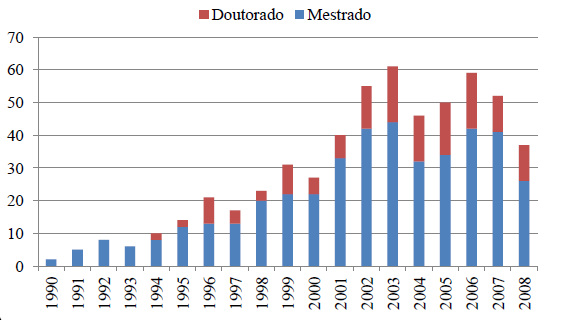
\includegraphics[scale=0.5]{figuras/figura-3}}
	}{
	\Fonte{os autores}
}
\end{figure}

Ou então figuras podem ser incorporadas de arquivos externos, como é o caso da \autoref{fig-grafico-1}. Se a figura que ser incluída se tratar de um diagrama, um gráfico ou uma ilustração que você mesmo produza, priorize o uso de imagens vetoriais no formato PDF. Com isso, o tamanho do arquivo final do trabalho será menor, e as imagens terão uma apresentação melhor, principalmente quando impressas, uma vez que imagens vetorias são perfeitamente escaláveis para qualquer dimensão. Nesse caso, se for utilizar o Microsoft Excel para produzir gráficos, ou o Microsoft Word para produzir ilustrações, exporte-os como PDF e os incorpore ao documento conforme o exemplo abaixo. No entanto, para manter a coerência no uso de software livre (já que você está usando LaTeX e abnTeX),  teste a ferramenta InkScape\index{InkScape}. ao CorelDraw\index{CorelDraw} ou ao Adobe Illustrator\index{Adobe! Illustrator}.  De todo modo, caso não seja possível  utilizar arquivos de imagens como PDF, utilize qualquer outro formato, como JPEG, GIF, BMP, etc.  Nesse caso, você pode tentar aprimorar as imagens incorporadas com o software livre \index{Gimp}Gimp. Ele é uma alternativa livre ao Adobe Photoshop\index{Adobe! Photoshop}.

\section{Usando Fórmulas Matemáticas}

\lipsum[2]

	\begin{equation}
		\begin{aligned}
			x = a_0 + \cfrac{1}{a_1
				+ \cfrac{1}{a_2
					+ \cfrac{1}{a_3 + \cfrac{1}{a_4} } } }
		\end{aligned}
	\end{equation}

\lipsum[3]

	\begin{equation}
		\begin{aligned}
			k_{n+1} = n^2 + k_n^2 - k_{n-1}
		\end{aligned}
	\end{equation}

\lipsum[4]

	\begin{equation}
		\begin{aligned}
			\cos (2\theta) = \cos^2 \theta - \sin^2 \theta
		\end{aligned}
	\end{equation}
	
\lipsum[5]

	\begin{equation}
		\begin{aligned}
			A_{m,n} =
			\begin{pmatrix}
			a_{1,1} & a_{1,2} & \cdots & a_{1,n} \\
			a_{2,1} & a_{2,2} & \cdots & a_{2,n} \\
			\vdots  & \vdots  & \ddots & \vdots  \\
			a_{m,1} & a_{m,2} & \cdots & a_{m,n}
			\end{pmatrix}
		\end{aligned}
	\end{equation}

\lipsum[6]

	\begin{equation}
		\begin{aligned}
			f(n) = \left\{ 
			\begin{array}{l l}
			n/2 & \quad \text{if $n$ is even}\\
			-(n+1)/2 & \quad \text{if $n$ is odd}
			\end{array} \right.
		\end{aligned}
	\end{equation}
	
\lipsum[7]

\section{Usando Algoritmos}

\lipsum[8]

\begin{algorithm}[h!]
	\SetSpacedAlgorithm
	\caption{\label{alg:algoritmo_de_colonica_de_formigas}Algoritmo de Otimização por Colônia de Formiga}
	\Entrada{Entrada do Algoritmo}
	\Saida{Saida do Algoritmo}
	\Inicio{
		Atribua os valores dos parâmetros\;
		Inicialize as trilhas de feromônios\;
		\Enqto{não atingir o critério de parada}{
			\Para{cada formiga}{
				Construa as Soluções\;
			}
			Aplique Busca Local (Opcional)\;
			Atualize o Feromônio\;
		}	
	}		
\end{algorithm}

\lipsum[9]

\section{Usando Código-fonte}

\lipsum[10]

\lstinputlisting[language=C++,caption={Hello World em C++}]{figuras/main.cpp}

\lipsum[11]

\begin{lstlisting}[language=Java,caption={Hello World em Java}]
public class HelloWorld {
	public static void main(String[] args) {
		System.out.println("Hello World!");
	}
}
\end{lstlisting}

\lipsum[11]

\section{Usando Teoremas, Proposições, etc}

Lorem ipsum dolor sit amet, consectetur adipiscing elit. Nunc dictum sed tortor nec viverra. consectetur adipiscing elit. Nunc dictum sed tortor nec viverra.

\begin{teo}[Pitágoras]
	Em todo triângulo retângulo o quadrado do comprimento da
	hipotenusa é igual a soma dos quadrados dos comprimentos dos catetos.
\end{teo}


Lorem ipsum dolor sit amet, consectetur adipiscing elit. Nunc dictum sed tortor nec viverra. consectetur adipiscing elit. Nunc dictum sed tortor nec viverra.

\begin{teo}[Fermat]
	Não existem inteiros $n > 2$, e $x, y, z$ tais que $x^n + y^n = z$
\end{teo}

Lorem ipsum dolor sit amet, consectetur adipiscing elit. Nunc dictum sed tortor nec viverra. consectetur adipiscing elit. Nunc dictum sed tortor nec viverra.

\begin{prop}
	Para demonstrar o Teorema de Pitágoras...
\end{prop}

Lorem ipsum dolor sit amet, consectetur adipiscing elit. Nunc dictum sed tortor nec viverra. consectetur adipiscing elit. Nunc dictum sed tortor nec viverra.

\begin{exem}
	Este é um exemplo do uso do ambiente exe definido acima.
\end{exem}

Lorem ipsum dolor sit amet, consectetur adipiscing elit. Nunc dictum sed tortor nec viverra. consectetur adipiscing elit. Nunc dictum sed tortor nec viverra.

\begin{xdefinicao}
	Definimos o produto de ...
\end{xdefinicao}

Lorem ipsum dolor sit amet, consectetur adipiscing elit. Nunc dictum sed tortor nec viverra. consectetur adipiscing elit. Nunc dictum sed tortor nec viverra.

\section{Usando Questões}


Lorem ipsum dolor sit amet, consectetur adipiscing elit. Nunc dictum sed tortor nec viverra. consectetur adipiscing elit. Nunc dictum sed tortor nec viverra.

\begin{questao}
	\item Esta é a primeira questão com alguns itens:
		\begin{enumerate}
			\item Este é o primeiro item
			\item Segundo item
		\end{enumerate}
	\item Esta é a segunda questão:
		\begin{enumerate}
			\item Este é o primeiro item
			\item Segundo item
		\end{enumerate}
	\item Lorem ipsum dolor sit amet, consectetur adipiscing elit. Nunc dictum sed tortor nec viverra. consectetur adipiscing elit. Nunc dictum sed tortor nec viverra.
		\begin{enumerate}
			\item consectetur
			\item adipiscing
			\item Nunc
			\item dictum
		\end{enumerate}
\end{questao}

\section{Citações}

\subsection{Documentos com três autores}

Quando houver três autores na citação, apresentam se os três, separados por ponto e vírgula, caso estes estejam após o texto. Se os autores estiverem incluídos no texto, devem ser separados por vírgula e pela conjunção "e".

\citeautoronline{tresautores}

\cite{tresautores}

\subsection{Documentos com mais de três autores}
Havendo mais de três autores, indica-se o primeiro seguido da expressão \textit{et al.} (do latim \textit{et alli}, que significa e outros), do ano e da página.

\citeautoronline{quatroautores}

\cite{quatroautores}

\subsection{Documentos de vários autores}

Havendo    citações    indiretas de    diversos    documentos    de    vários    autores, mencionados  simultaneamente e  que  expressam  a  mesma  ideia,  separam-se  os  autores  por ponto e vírgula, em ordem alfabética.

\cite{tresautores, quatroautores}

\section{Notas de Rodap\'{e}}

Deve-se utilizar o sistema autor-data para as  citações no texto e o numérico para notas explicativas\footnote{Veja - se como exemplo desse tipo de abordagem o estudo de Netzer (1976)}. As notas de rodapé podem e devem ser alinhadas, a partir da segunda linha da mesma nota, abaixo da primeira letra da primeira palavra, de forma a destacar o expoente \footnote{Encontramos  esse  tipo  de  perspectiva  na  2ª  parte  do  verbete  referido  na  nota  anterior,  em  grande  parte  do estudo de Rahner (1962).} e sem espaço entre elas e com fonte menor (tamanho 10).


	\chapter{Resultados}
\label{chap:resultados}

\lipsum[2]

\section{Resultados do Experimento A}
\label{sec:resultados-do-experimento-a}

\lipsum[3]

\section{Resultados do Experimento B}
\label{sec:resultados-do-experimento-b}

\lipsum[4]
	\chapter{Conclusões e Trabalhos Futuros}
\label{chap:conclusoes-e-trabalhos-futuros}

\lipsum[2]
\lipsum[34]

\section{Contribuições do Trabalho}
\label{sec:contribuicoes-do-trabalho}

\lipsum[3]

\section{Limitações}
\label{sec:limitacoes}

\lipsum[4]

\section{Trabalhos Futuros}
\label{sec:trabalhos-futuros}

\lipsum[5]





	
	%Elementos pós-textuais	
	\bibliography{elementos-pos-textuais/referencias}
	%\imprimirglossario	
	%\imprimirapendices
		% Adicione aqui os apendices do seu trabalho
	%	\apendice{Lorem Ipsum}
\label{ap:lorem-ipsum}

\lipsum[1]
	%	\apendice{Modelo de Capa}
\label{ap:modelo-de-capa}

\lipsum[1]

	%	\apendice{Termo de Fiel Depositário}
\label{ap:termo-de-fiel-depositario}

\noindent \textbf{Pesquisa:} ANÁLISE DA MORTALIDADE INFANTIL COM MALFORMAÇÕES CONGÊNITAS.

\noindent Pelo presente instrumento que atende às exigências legais, a Sra. Maria Consuelo Martins Saraiva, ``fiel depositário'' com o cargo de Secretária Municipal de Saúde de Iracema, após ter tomado conhecimento do protocolo de pesquisa intitulado: ANÁLISE DA MORTALIDADE INFANTIL COM MALFORMAÇÕES CONGÊNITAS. Analisando a repercussão desse estudo no contexto da saúde pública e epidemiologia, autoriza Karla Maria da Silva Lima, enfermeira, aluna do Curso de Mestrado Acadêmico em Enfermagem da Universidade Estadual do Ceará (UECE), sob orientação do Prof. Dr. José Maria de Castro, da UECE, ter acesso aos bancos de dados do Sistema de Informação sobre Nascidos Vivos e do Sistema de Informação sobre Mortalidade da Secretaria Municipal de Saúde de Iracema, objeto deste estudo, e que se encontram sob sua total responsabilidade. Fica claro que o Fiel Depositário pode a qualquer momento retirar sua AUTORIZAÇÃO e ciente de que todas as informações prestadas tornar-se-ão confidenciais e guardadas por força de sigilo profissional, assegurando que os dados obtidos da pesquisa serão somente utilizados para estudo.	
	%\imprimiranexos
		% Adicione aqui os anexos do seu trabalho
	%	\anexo{Exemplo de Anexo}
\label{an:exemplo-de-anexo}

\lipsum[13]		
	%	\anexo{Dinâmica das classes sociais}
\label{an:dinamica-das-classes-sociais}

\lipsum[14]
\index{AAA}
	%\imprimirindice

\end{document}